\chapter{LaTeX Tutorial}

This section provides a brief tutorial on how to use LaTeX to insert links, write mathematical equations, and include figures in your thesis. These are some of the essential skills for formatting your document effectively.

\section{Inserting Links}
To insert a hyperlink in your LaTeX document, use the \texttt{hyperref} package. This package allows you to add clickable links to URLs, references, and even email addresses. Here’s how you can use it:

\begin{itemize}
    \item \textbf{Inline Math Mode}: For short formulas within text, enclose the math expression with dollar signs:
    \begin{verbatim}
    This is an inline equation:
    $ x = \frac{-b \pm \sqrt{b^2 - 4ac}}{2a}$.
    \end{verbatim} 
    which renders as \( x = \frac{-b \pm \sqrt{b^2 - 4ac}}{2a} \).

    \item \textbf{Displayed Math Mode}: For larger equations or equations that need to be centered on their own line, you can use the `equation` environment.

    \begin{verbatim}
    \begin{equation}
        x = \frac{-b \pm \sqrt{b^2 - 4ac}}{2a}
    \end{equation}
    \end{verbatim}

    This will display the equation on its own line and automatically number it, like this:
    \begin{equation}
    x = \frac{-b \pm \sqrt{b^2 - 4ac}}{2a}
    \end{equation}
    
    \item \textbf{Multiple Equations with Alignment}: To display multiple equations and align them at specific points, such as the equals sign, you can use the `align` environment, which requires the `amsmath` package.
    
    First, add the following to your preamble:
    \begin{verbatim}
    \usepackage{amsmath}
    \end{verbatim}
    
    Then, use the `align` environment:
    \begin{verbatim}
    \begin{align}
        x &= \frac{-b + \sqrt{b^2 - 4ac}}{2a} \\
        x &= \frac{-b - \sqrt{b^2 - 4ac}}{2a}
    \end{align}
    \end{verbatim}

    This will display two equations aligned at the equals sign, like this:
    \[
    x = \frac{-b + \sqrt{b^2 - 4ac}}{2a}
    \]
    and
    \[
    x = \frac{-b - \sqrt{b^2 - 4ac}}{2a}
    \]
    
    The `align` environment allows you to align multiple equations and gives each equation its own number.
\end{itemize}




\section{Tables with \texttt{natbib}}
The \texttt{natbib} package is commonly used for citation management in LaTeX, but it does not directly relate to tables. However, you can use it to cite sources in table captions.

To include the \texttt{natbib} package in your document, add the following in the preamble:

\begin{verbatim}
\usepackage{natbib}
\bibliographystyle{plainnat} % Or another style like abbrvnat
\end{verbatim}

To create a table, use the \texttt{tabular} environment:

\begin{verbatim}
\begin{table}[h]
    \centering
    \begin{tabular}{|c|c|c|}
        \hline
        Column 1 & Column 2 & Column 3 \\
        \hline
        Data 1 & Data 2 & Data 3 \\
        Data 4 & Data 5 & Data 6 \\
        \hline
    \end{tabular}
    \caption{Example Table \citep{author2025book}}
    \label{tab:example}
\end{table}
\end{verbatim}

This will create a table with three columns, as follows:


\begin{table}[h]
    \centering
    \begin{tabular}{ccc}
        \hline
        Column 1 & Column 2 & Column 3 \\
        \hline
        Data 1 & Data 2 & Data 3 \\
        Data 4 & Data 5 & Data 6 \\
        \hline
    \end{tabular}
    \caption{Example Table \citep{author2025book}}
    \label{tab:example}
\end{table}

% with citations in the caption. The \texttt{\citep} command from \texttt{natbib} allows in-text citations in the caption.


\section{Adding Pictures}
To include images, use the \texttt{graphicx} package:

\begin{verbatim}
\usepackage{graphicx}
\end{verbatim}

Example:

\begin{verbatim}
\begin{figure}[h]
    \centering
    
\includegraphics[width=0.5\textwidth]{assets/images.png}
    \caption{The emblem of the University of Limerick.}
    \label{fig:image}
\end{figure}
\end{verbatim}



\begin{figure}[h]
    \centering
    
\includegraphics[width=0.5\textwidth]{assets/images.png}
    \caption{The emblem of the University of Limerick.}
    \label{fig:image}
\end{figure}


To reference this image use \texttt{ref} as follows:


\begin{verbatim}
As shown in Figure \ref{fig:image}, the example...
\end{verbatim}




\section{Drawing with \texttt{TikZ}}

The \texttt{TikZ} package allows for drawing detailed scientific diagrams such as spacetime graphs. To use it, include the package  \texttt{tikz} in the preamble.

You can create various shapes and diagrams using LaTeX. For example, here is a spacetime diagram with vertical worldlines, light signals, and annotations. To find more information on how to create a similar diagram, visit \href{https://tikz.net/relativity_minkowski_diagram/}{this link}.

\begin{verbatim}
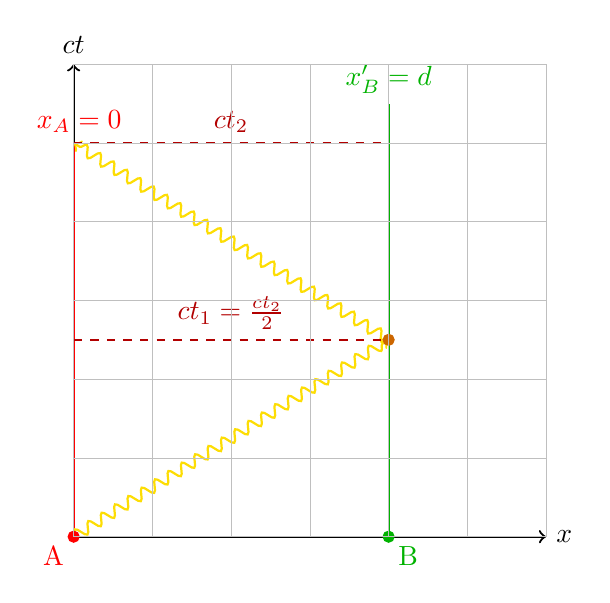
\begin{tikzpicture}
    % Axis
    \draw[->, thick] (0,0) -- (0,6) node[above] {\(ct\)};
    \draw[->, thick] (0,0) -- (6,0) node[right] {\(x\)};
    
    % Worldlines
    \draw[thick, red] (0,0) -- (0,5) node[above, xshift=2pt] 
    {\textcolor{red}{\(x_A = 0\)}};
    \draw[thick, green!70!black] (4,0) -- (4,5.5) node[above] 
    {\textcolor{green!70!black}{\(x'_B = d\)}};
    
    % Light paths
    \draw[->, thick, yellow!80!orange, 
    decorate, decoration={snake, amplitude=0.7mm, segment length=2mm}]
        (0,0) -- (4,2.5);
    \draw[->, thick, yellow!80!orange, 
    decorate, decoration={snake, amplitude=0.7mm, segment length=2mm}]
        (4,2.5) -- (0,5);

    % Dotted lines
    \draw[dashed, thick, red!70!black] 
    (0,2.5) -- (4,2.5) node[midway, above] 
    {\(ct_1 = \frac{ct_2}{2}\)};
    \draw[dashed, thick, red!70!black] 
    (0,5) -- (4,5) node[midway, above] {\(ct_2\)};
    
    % Events
    \filldraw[red] (0,0) circle (2pt) node[below left] {A};
    \filldraw[green!70!black] (4,0) circle (2pt) node[below right] {B};
    \filldraw[orange!80!black] (4,2.5) circle (2pt);

    % Grid (optional)
    \draw[step=1cm, lightgray, very thin] (0,0) grid (6,6);
\end{tikzpicture}
\end{verbatim}

This renders the following diagram:

\begin{figure}[h]
\centering
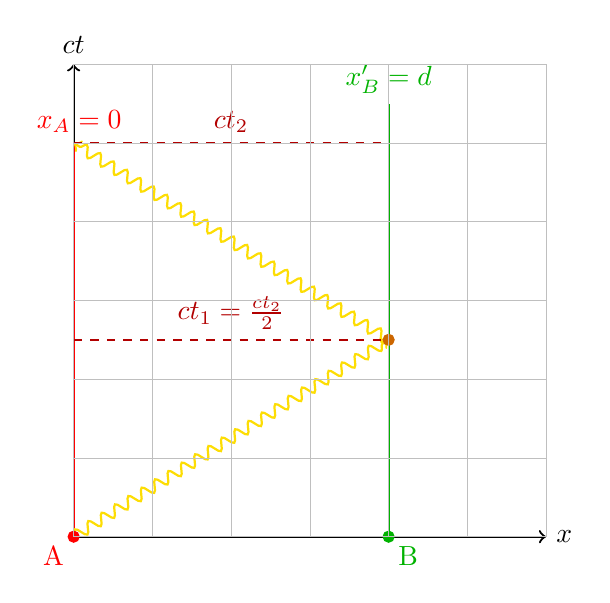
\begin{tikzpicture}
    % Axis
    \draw[->, thick] (0,0) -- (0,6) node[above] {\(ct\)};
    \draw[->, thick] (0,0) -- (6,0) node[right] {\(x\)};
    
    % Worldlines
    \draw[thick, red] (0,0) -- (0,5) node[above, xshift=2pt] {\textcolor{red}{\(x_A = 0\)}};
    \draw[thick, green!70!black] (4,0) -- (4,5.5) node[above] {\textcolor{green!70!black}{\(x'_B = d\)}};
    
    % Light paths
    \draw[->, thick, yellow!80!orange, decorate, decoration={snake, amplitude=0.7mm, segment length=2mm}]
        (0,0) -- (4,2.5);
    \draw[->, thick, yellow!80!orange, decorate, decoration={snake, amplitude=0.7mm, segment length=2mm}]
        (4,2.5) -- (0,5);

    % Dotted lines
    \draw[dashed, thick, red!70!black] (0,2.5) -- (4,2.5) node[midway, above] {\(ct_1 = \frac{ct_2}{2}\)};
    \draw[dashed, thick, red!70!black] (0,5) -- (4,5) node[midway, above] {\(ct_2\)};
    
    % Events
    \filldraw[red] (0,0) circle (2pt) node[below left] {A};
    \filldraw[green!70!black] (4,0) circle (2pt) node[below right] {B};
    \filldraw[orange!80!black] (4,2.5) circle (2pt);

    % Grid (optional)
    \draw[step=1cm, lightgray, very thin] (0,0) grid (6,6);
\end{tikzpicture}
\caption{Spacetime diagram showing light signal exchange between two observers.}
\label{fig:spacetimetikz}
\end{figure}

\newpage
\section{Using Citations}
To cite sources, use the \texttt{biblatex} package:

\begin{verbatim}
\usepackage{biblatex}
\addbibresource{references.bib}
\end{verbatim}

\subsection{Inline Citation Example}
Use \texttt{\textbackslash cite} to refer to an author within the text:

\begin{verbatim}
According to \cite{author2025book}, books are important.
\end{verbatim}

\subsection{Parenthetical Citation Example}
Use \texttt{\textbackslash parencite} to place citations in parentheses:

\begin{verbatim}
Books are an important source of knowledge \parencite{author2025book}.
\end{verbatim}

To list all references, add:

\begin{verbatim}
\printbibliography
\end{verbatim}

\textcolor{blue}{This is an example of using color in your document~\cite{author2024article,author2023conference}.}
